% omci.tex:

\chapter{OPTICAL MAMMOGRAPHY CO-IMAGER (OMCI)} % all caps please
\label{chap:omci}
OMCI is a high-density standalone hybrid diffuse optical breast tomography system aimed at supplementing any structural breast imaging technique. The device integrates mechanical compression of the breast to resemble clinical mammography, uses a frequency-domain subsystem for recovering absolute tissue optical properties, uses a wide-field trans-illumination diffuse optical system to generate three-dimensional tomographic images, and recovers high-resolution meshes of the breast surface. Although OMCI is composed of four separate subsystems working in tandem, in this chapter, we will provide an overall instrument characterization as well as further elaborate the dual-camera structured light imaging (SLI) breast shape acquisition system used for improving diffuse optical tomography image reconstructions.

% challenge and application
%innovation and significance

\section{Introduction} %significance
\label{chap:omci:introduction}
Breast cancer is the most commonly diagnosed cancer in women worldwide with an estimated 1,918,030 new cases in 2022 in the United States alone~\cite{Siegel2022}. It is the second leading cause of death among women with a 2.6\% chance of dying. Multiple breast cancer imaging modalities are employed in the clinics for screening and diagnostics based mainly on structural and functional tissue characteristics. 
Modalities such as magnetic resonance imaging (MRI) and positron emission tomography (PET) are infrequently due to their high cost, limited specificity, and use of radioactive isotopes. X-ray mammography, along with its three-dimensional extension, digital breast tomosynthesis (DBT), are the primary breast cancer screening techniques~\cite{Secretan2015} used for early detection to reduce mortality rates~\cite{Tabar2003}. Despite its recommendation for screening, not only does x-ray mammography expose patients to ionizing radiation but it also suffers from a high false-positive diagnostic rate~\cite{Tabar2003, Elmore1998}. The technique lacks both strong structural contrast between healthy and tumor tissue and the ability to quantify tissue functions to assess benign versus malignancy~\cite{Leff2008}. These limitations have led researchers to investigate using diffuse optical tomography (DOT) techniques to characterize the breast tumor's physiology to lower false-positive diagnoses. 

Unlike x-ray mammography, DOT is an imaging modality that uses non-ionizing near-infrared (NIR) radiation to yield three-dimensional (3-D) maps of the optical properties of illuminated tissue~\cite{Boas2001, Dehghani2009, Yamada2014, Hoshi2016}. Biological tissues' primary absorbers in the spectral window from around 600 to 1000~nm have relatively low absorption, allowing NIR light to penetrate through centimeters of tissues~\cite{Gibson2005}. This allows the quantification of physiological properties such as hemoglobin concentration, blood volume, and blood oxygen saturation~\cite{Leff2008, Boas2001}. Malignant tumors generally demand a greater blood supply than their surrounding tissues, leading to increased light absorption that can be delineated using spectroscopy and imaging methods, making DOT particularly useful for breast cancer imaging diagnosis~\cite{Wang2022, Vavadi2014, Flexman2013, Choe2009, Taroni2005}. Unfortunately, DOT images are known for low spatial resolution largely caused by the high scattering properties of biological tissues~\cite{Boas2001}. The typical coarse spatial sampling of current DOT setups and their sensitivity to tissue-optode coupling coefficients~\cite{Schweiger2007} lead to inaccurate representations of tissue composites and low spatial resolution images~\cite{Durduran2010}.

The low spatial resolution of DOT~\cite{Li2010} can be improved by a multi-modal approach with x-ray mammography~\cite{Zimmermann2017, Deng2015, Deng2015a, Fang2009a}. The high scattering present in the breast tissue redirects photons to traverse large overlapping probing volumes before their detection, greatly reducing the locality of the measurements and resulting in blurry images. Mathematically, this is reflected as the severe ill-posedness of the inverse problem. Parallel-plate compression of breast tissues has been used in an x-ray mammography scan to minimize overlapping tissues and has also been explored for a number of standalone~\cite{Choe2009, Culver2003} and multi-modal DOT breast imaging systems~\cite{ZhuReview2020, Fang2009a, Krishnaswamy2012}. Multi-modal imaging approaches have been developed by leveraging tissue structural priors obtained from high-resolution imaging methods such as magnetic resonance imaging~\cite{Ghussein2013,Ntziachristos2002} and ultrasound~\cite{Zhu2010}. These approaches allow to better constrain the inverse problem solution and reduce the impact of data acquisition artifacts to provide higher image quality with more accurate functional tissue physiology representation. In particular, co-registration of DOT with structural information from x-ray technologies is of special interest due to its high-resolution, relative low-cost, and high prevalence as the primary clinical standard for early breast cancer diagnosis.

Additionally, the DOT reconstruction can also be improved through constraining the inverse problem through more accurate surface representations of the breast. Obtaining breast surface information to aid quantitative analysis of imaging data has garnered interest from a number of applications, including digital breast tomosynthesis (DBT)~\cite{Rodriguez2017} and magnetic resonance imaging (MRI) scans~\cite{Pallone2014, Ortiz2012}. For multi-modal DOT systems, the 3-D shape of the breast can be estimated using the structural imaging modality such as DBT~\cite{Fang2011} or MRI~\cite{Brooksby2006}. When a 3-D imaging modality is not available, two-dimensional (2-D) mammography~\cite{Deng2015a} has also been used to provide the shape information. In such case, a simple way to recover a 3-D breast surface is to extrude the 2-D breast contour along the compression axis~\cite{Kruger2013, Kalbhen1999}, or sweep the 2-D breast contour along the contour line extracted from an orthogonal view~\cite{Kita1998}. These methods either rely on assumptions about the 3-D location of certain features (e.g. mamilla position) or assume a constant curvature of the breast along the sweeping direction. For more accurate reconstructions of tissue optical properties, especially near the surface, measuring 3-D breast surface accurately can be greatly beneficial.

Accurately acquiring breast 3-D surface shapes has gained clinical acceptance due in large part to the plastic and reconstructive surgery communities~\cite{Chang2015, Losken2005}. The two prominent techniques for 3-D breast surface imaging are stereophotogrammetry and laser scanning~\cite{Yang2015}. Stereophotogrammetry works by overlaying multiple images of an object taken from different view angles and triangulating the location of the object based on matching features in the multiple images~\cite{Ju2016, Galdino2002, FangOSA2012}. In addition to requiring multiple cameras to increase accuracy~\cite{Henseler2012}, this technique is also heavily influenced by lighting conditions since features need to be extracted from multiple viewpoints~\cite{Henseler2011}. Another limitation is the ``ptosis error'' seen during scanning of ptotic or larger breasts~\cite{Nahabedian2003}. This arises due to the small field of view of stereophotogrammetry systems, leading to inaccuracies in breast surface and volume estimations due to the portions of the breast that are not illuminated. Laser scanning is a surface imaging technique in which rays from a laser beam are reflected off an object and detected by a detector~\cite{Kovacs2006}. Although laser-based acquisition systems can produce more accurate surfaces~\cite{Kovacs2006b}, these systems tend to be expensive~\cite{Kovacs2007, Koch2011} and require the need for very precise setups~\cite{Thomson2009}. Recently, the use of patterned-lasers and orientation-sensitive detectors has led to an increase in portable 3-D laser scanning devices~\cite{Kuzminsky2012}. While low-cost laser-based depth sensors have been widely deployed in game consoles such as Xbox or PlayStation, they are only designed to achieve relatively low spatial accuracy compared to dedicated 3-D scanners. Still, patterned-laser-based surface acquisition systems generally require a minimum scanner-to-target distance of 35~cm~\cite{Ametek2002, Artec3D2022}. Additionally, their typical housing is too large to fit between mammography compression plates~\cite{Artec3D2022, Pallone2014}. Bulky instrumentation and long minimum working distance requirements make stereophotogrammetry and laser scanning techniques infeasible in the confined, low-light mammography setting. 

Another widely used 3-D surface acquisition technique is structured light imaging (SLI)~\cite{Yang2020, Zhang2018}. SLI works by illuminating an object with two-dimensional spatially varying patterns with a projector and capturing images from the illuminated object using cameras~\cite{Geng2011}. The distortion of the specially designed patterns provides information regarding the shape of the object. Calibration of the camera-projector system is easily done by capturing images of a known planar pattern (e.g. a checkerboard). With the ability to use off-the-shelf components, a simple setup with a single projector and camera, and a robust and simple calibration method, SLI is positioned to provide accurate, fast, and cost-effective breast surface scanning~\cite{Yang2020}. However, similar to most patterned-laser surface scanners, commercially available SLI systems have long minimal working distance requirements and large assemblies that cannot readily fit within the confined mammography compression plates~\cite{Zhang2018, Rodriguez2017}.

Our approach to lowering false-positive diagnoses is two-fold. We first aim to improve DOT reconstruction through more accurate representations of the compressed breast. Second, we develop a standalone DOT breast imaging system that leverages structural information through the registration of the DOT reconstruction with prior x-ray mammographies. The idea of independent acquisition of optical data and x-ray images foresees an attractive scenario for a wider clinical adoption of DOT by simplifying its regulatory pathways. In this respect, our group has recently explored the feasibility of integrating previously acquired x-ray mammography images into the DOT reconstruction algorithm~\cite{Deng2015} resulting in improved spatial details in the optical images and robust optical property estimation all while avoiding the necessity of sophisticated breast deformation algorithms\cite{Azar2007}.

Our group has pioneered the development of multi-modal DOT and digital breast tomosynthesis (DBT) instrumentation over the last decade~\cite{Fang2009,Zimmermann2017}. These approaches aim to hybridize DOT with commercially available DBT devices in order to increase the research impact of DOT methods in clinical environments. Along these lines, our group~\cite{Carp2006,Carp2008,Carp2013} and others~\cite{Wang2008,Fournier2009,Alabdi2011} have demonstrated the feasibility of stand-alone DOT systems to resolve dynamic physiological changes in breast tissue under mechanical compression, yielding to a potential synergistic scenario with the required mechanical compression of DBT. Building upon our decade-long research, we have developed OMCI---a high performance optical mammography co-imager to bring seamless multi-modal data fusion and, consequently, improved breast cancer characterization to all existing (or future) mammography scanners. 

In this chapter, we first describe the overall OMCI instrument and its subsystems. We follow this with a description how the subsystem data is integrated into our reconstruction algorithm. We then describe the design of the SLI breast scanner and detail the methods for adaptive illumination for subject-specific skin tones as well as approaches to reduce specular reflection from the compression plates. Next, we compare several traditional surface acquisition methods that leverage mammography images against our SLI-based breast surface acquisition system and quantify the impact of improved breast surface acquisition on the recovery of breast lesions using a series of simulations. Finally, we demonstrate the performance of OMCI through a set of measurements on heterogeneous and 3-D printed phantoms.



\section{Methods}
\label{chap:omci:methods}

%%% Subsection %%%
\subsection{OMCI Instrument}
An overview of the OMCI system is shown in Figure~\ref{fig:OMCISystem}. The instrument integrates a mechanical motion stage, a sensor cluster for auxiliary monitoring, and three optical subsystems all controlled and monitored using an in-house developed software through an Arduino board (Arduino Uno, Arduino, Italy). 

\begin{figure}[]
    \begin{center}
    \subfigure[]{\label{fig:OMCISystemA}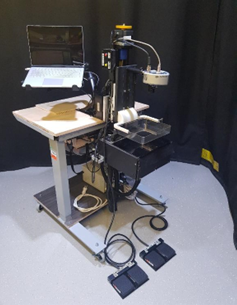
\includegraphics[width=.4\textwidth]{fig/omci/OMCISystemImage_1.png}}
    \subfigure[]{\label{fig:OMCISystemB}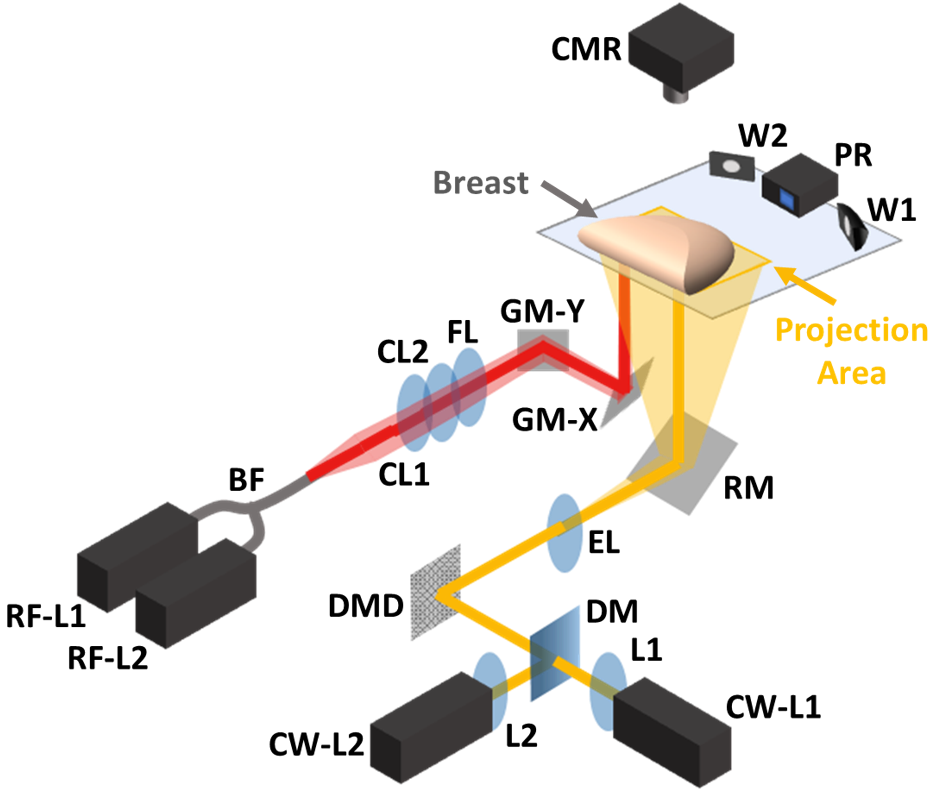
\includegraphics[width=.5\textwidth]{fig/omci/OMCISystemSketch.png}}
    \end{center}
    \caption{(a) The OMCI system in its fully compressed state. (b) A schematic of the OMCI components and subsystems. The wide field optical system consists of: CW lasers (CW-L1/2), lenses (L1/2), a dichroic mirror (DM), a digital micromirror Device (DMD), an expansion lens (EL), a reflection mirror (RM), and the measuring camera (CMR). The frequency domain subsystem consists of: RF lasers (RF-L1/2), a bifurcation fiber (BF), collimation lenses (CL1/2), a focusing lens (FL), dual-axis galvo mirrors (GM-X/Y), and a detection fiber located above the breast (RFD). The structured light imaging subsystem consists of: two webcams (W1/2) and a pattern illumination projector (PR).} 
    \label{fig:OMCISystem}
\end{figure} 

\subsubsection{Mechanical stage and auxiliary sensors suite}
OMCI is composed of a linear and rotary stage. The breast is compressed by a pair of acrylic plates, with one plate mounted at the stationary end of a linear stage (MN10-0160-M02-31 BiSlide, Velmex, NY, USA). The bottom paddle also serves as a cover for the OMCI projection box which encloses most of the components of the system. An acrylic mammography compression paddle is mounted on the moving gantry of the linear stage, allowing for a plate separation ranging from 300~mm (fully released) to 0~mm (fully closed). A linear encoder (ETI Systems, Carlsbad, CA, USA) is connected between the pair of compression plates to measure their separation. The entire breast compression assembly is mounted on a rotatory table (306045-1-s-M04-C376, Lintech, Monrovia, CA, USA), controlled by a foot paddle to permit mammography-like lateral-oblique compression. Each stage is actuated by a stepper motor (NEMA 34 PK296 Stepper Motor, Oriental Motor Corporation, MA, USA) controlled through a motor driver interface (VXM-2, Velmex Inc., USA). In addition to the linear encoder, sensor cluster encompasses two limit switches (BiSlide Push Button, Velmex Inc., NY, USA) in the translation stage, a reed switch in the rotary stage (L06 Non-Contact Reed Switch, LinTech Motors, CA, USA), and four load sensors (SEN-10245, SparkFun, CO, USA) inside the OMCI projection box. The limit and reed switches serve to confine the degree of motion of the linear and rotation stages while the pressure sensor informs of the compression force exerted on the breast. This design specifically enables registration of structural information from separately acquired mammography scans with the DOT images using the methods detailed in our previous studies~\cite{Deng2015}.

\subsubsection{Galvo-based frequency-domain subsystem}
\label{sec:RF}
A custom-built frequency-domain (FD) spectroscopy device~\cite{Zimmermann2016} was employed for bulk tissue optical properties estimation. The FD subsystem consist of two laser modules at 690~nm (HL6750MG, Thorlabs GmbH, Germany) and 830~nm (HL8338MG, Thorlabs GmbH, Germany) modulated at 67.5 and 75~MHz, respectively, with an average power of 25~mW and a modualtion depth of 90\%. Each laser module is coupled to one of the two input fibers of a 400~$\mu$m core bifurcated fiber bundle (BFY400LS02, Thorlabs GmbH, Germany). The single fiber light output was collimated and focused to a 3~mm source spot at the surface of the bottom compression paddle through a collection of optical lenses (C610TME-B, LA4647-B and AC254-300-B, Thorlabs GmbH, Germany). Frequency multiplexing of the light sources allows for simultaneous dual-wavelength illumination. A dual-axis galvo motor system (GVS002, Thorlabs GmbH, Germany) was utilized to position the light source at nine different positions along a 6~cm length linear trace (parallel to the chest wall). A single customized 1000~$\mu$m core detection optical fiber (FP1000ERT, Thorlabs GmbH, Germany), located directly above the last source position and attached to the top compression paddle, was used to collect the diffuse transmitted light and deliver it to a frequency-domain detector (C5331-04, Hamamatsu, Japan) for subsequent frequency-domain analysis to subtract amplitude and phase parameters. Assuming an average sample thickness of 6~cm, the source-detector (SD) separation ranges from 6 to 8.5~cm.

\subsubsection{Ultra-high-density wide-field tomography subsystem}
\label{sec:WF}
The wide-field (WF) tomography subsystem utilizes a modified projector (P300 Neo, Aaxa Technologies, USA) for dual-wavelength illumination. The built-in collimation lenses and dichroic mirrors were removed. The LED triplet was replaced by a pair of high-power laser modules at 660~nm and 830~nm and a single dichroic longpass filter (69-882, 750~nm cut-on, Edmund Optics, USA). The laser on/off switch is controlled by the OMCI software using an Arduino board (Arduino UNO, Arduino, Italy) interface. The modified projector produces a full illumination area of $11\times6~cm^2$ at the surface of the bottom compression paddle with a total output power of 26~mW (0.39~mW/cm$^2$) at 660~nm and 10~mW (0.15~mW/cm$^2$) at 830~nm. The projector's gamma function was corrected to account for the non-linearities of the projected light intensities. The light transmitted through the sampled tissue is collected by a 14-bit EMCCD camera (Andor Luca R, Oxford Instruments;, U.K) fixed at 45~cm from the top compression paddle using a 200~ms exposure time. A set of 32 sliding-bar patterns per wavelength are used to illuminate the targeted sample from underneath.

%%% Subsection %%%
\subsection{Dual-camera SLI breast surface scanning system}
\label{sec:sli}
\begin{figure}
	\begin{center}
	\subfigure[]{\label{fig:mammography_top}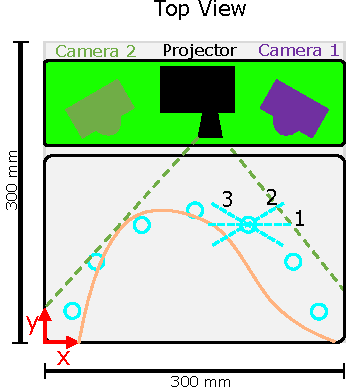
\includegraphics[height=5cm]{fig/omci/mammography_top.pdf}}
	\subfigure[]{\label{fig:mammography_side}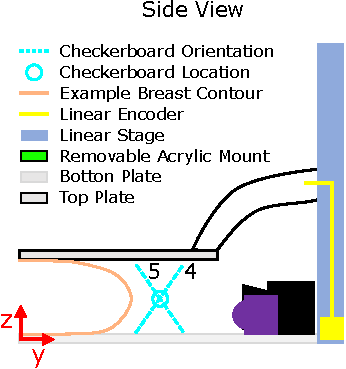
\includegraphics[height=5cm]{fig/omci/mammography_side.pdf}}
	\subfigure[]{\label{fig:mammography_setup}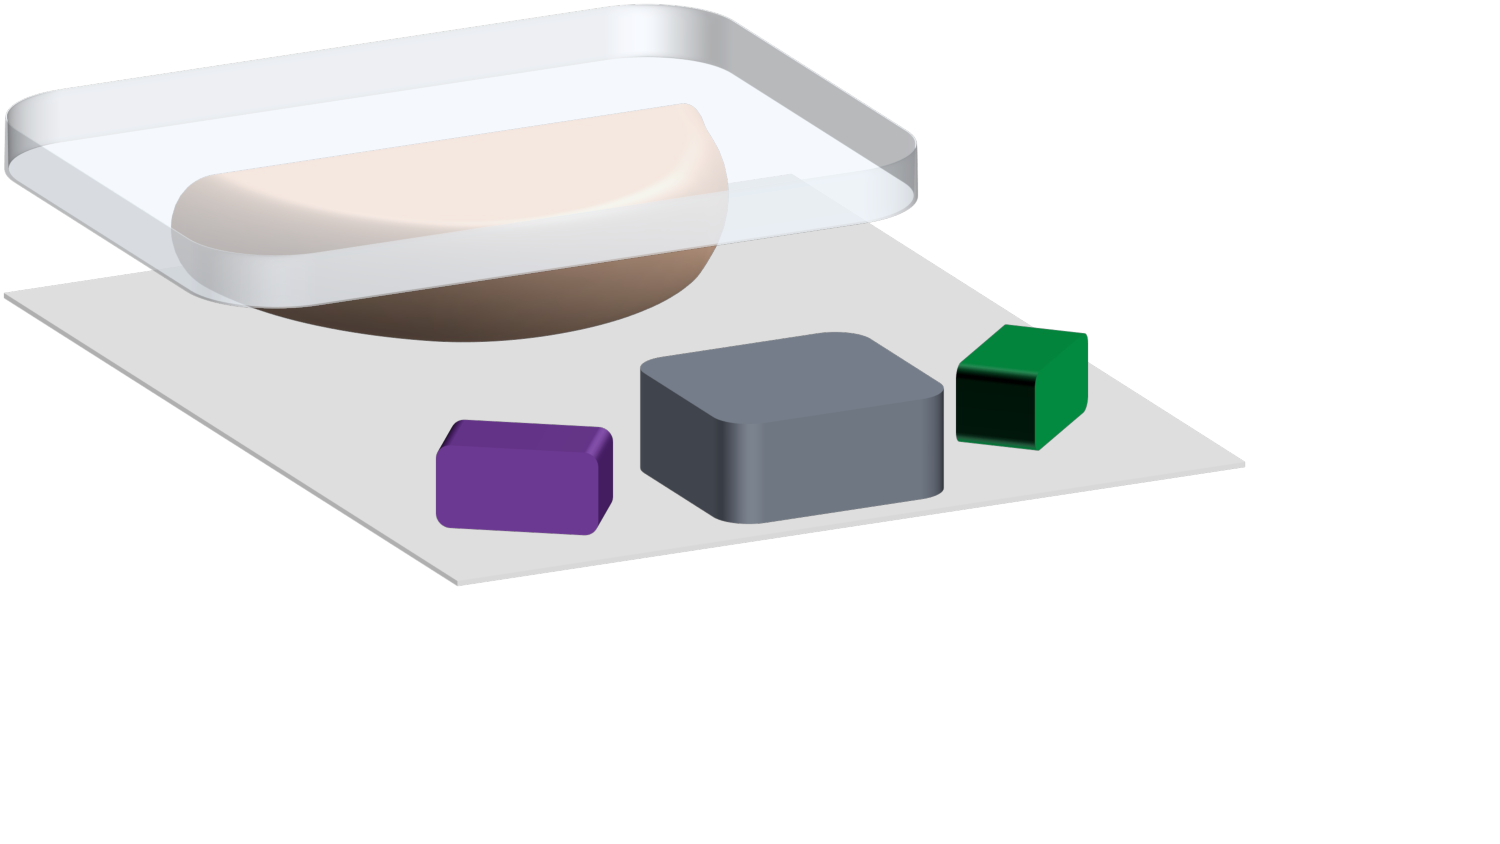
\includegraphics[width=5cm]{fig/omci/sli_model.pdf}}
	\end{center}
	\caption{ (a) Top-view of the breast compression compartment -- upper: SLI system; bottom: horizontal cross-section (orange line) of the compressed breast with blue circles indicating the placement of the checkerboard used for system calibration. Numbers 1-5 indicate the 5 board orientations repeated at each location for calibration. (b) Side-view of the breast compression plates, showing the linear translation stage (blue bar on the right) and a linear encoder (in yellow), and  (c) 3-D rendering of the SLI system, an acrylic bottom plate and an acrylic compression paddle (top). } 
	\label{fig:mammographysetup}
\end{figure} 
The SLI system is embedded between the compression plate to provide accurate measurement of the breast surface [Fig.~\ref{fig:mammography_setup}].This low-profile SLI scanner has a dimension of 30$\times$10$\times$4.8~cm$^3$, and is fixated on a stationary compression plate, on the side facing the patient's breast [Fig.~\ref{fig:sli_setup}]. It consists of a central projector (P2-B DLP Pico Projector, AAXA Technologies, Irvine, CA, USA) and two USB cameras (C525, Logitech, Lausanne, Switzerland) to reconstruct a 3-D surface of the compressed breast. The SLI scanner is designed to have a relatively short scanner-to-target distance, typically less than 15~cm, and a vertical profile of less than 3~cm to permit scanning breasts with a wide range of sizes. A laptop is used to control the data acquisition, including illumination pattern generation, projection, camera image acquisition, and translation stage control via an interface written in MATLAB (R2017b, Mathworks, Natick, MA, USA).

Gray-code based binary patterns~\cite{Inokuchi1984} are sequentially illuminated onto the breast surface and captured using both USB cameras. These patterns are characterized by their pattern order, $P$. A pattern set of $P=3$ results in 3 sequences which are a reflected binary of the previous (``01'', ``0110'', and ``01100110''). Four bar patterns are created for each sequence (a horizontal black and white bar pattern, a vertical black and white bar pattern, and the complimentary pattern of each)~\cite{Sels2019}. The digits correspond to the white (``1'') and black (``0'') bars. In addition, a full-bright (white) and full-dark (black) pattern are added to each pattern set. Thus, a pattern set of $P=3$ results in $4\times P+2$ illumination bar patterns. Complimentary Gray-code based illumination pattern sets are used due to their robustness to decoding errors~\cite{Moreno2012}. The two USB cameras have overlapping field-of-views and sequentially capture images of the breast during each illumination pattern at an exposure time of 250~ms. Dual-camera simultaneous acquisition allows the SLI system to capture the curved surface of breasts of varied sizes without moving components. 

\subsubsection{Special data acquisition considerations}\label{sec:special}
% skin tone
Skin tone differences are known to affect light-based surface reconstruction accuracy, especially in low-light settings. To account for skin tone variations, the normalized illumination patterns are multiplied by a scaling factor $\alpha$ ranging from 0 to 1 to prevent camera saturation. The scaling factor for a camera is calculated prior to data acquisition by first illuminating a full-bright pattern with $\alpha=1$ onto the breast and capturing a single image using the camera. If the maximum pixel value of the captured image is above a preset threshold, $\alpha$ is decreased and the breast is re-illuminated with a full-bright pattern multiplied by the new $\alpha$ value. This procedure is repeated until the maximum pixel value of the captured image is less than 95\% of the camera's maximum allowable pixel value. This entire procedure takes an estimated 8 seconds to complete and is repeated for each camera.

\begin{figure}
	\begin{center}
	\subfigure[]{\label{fig:sli_setup}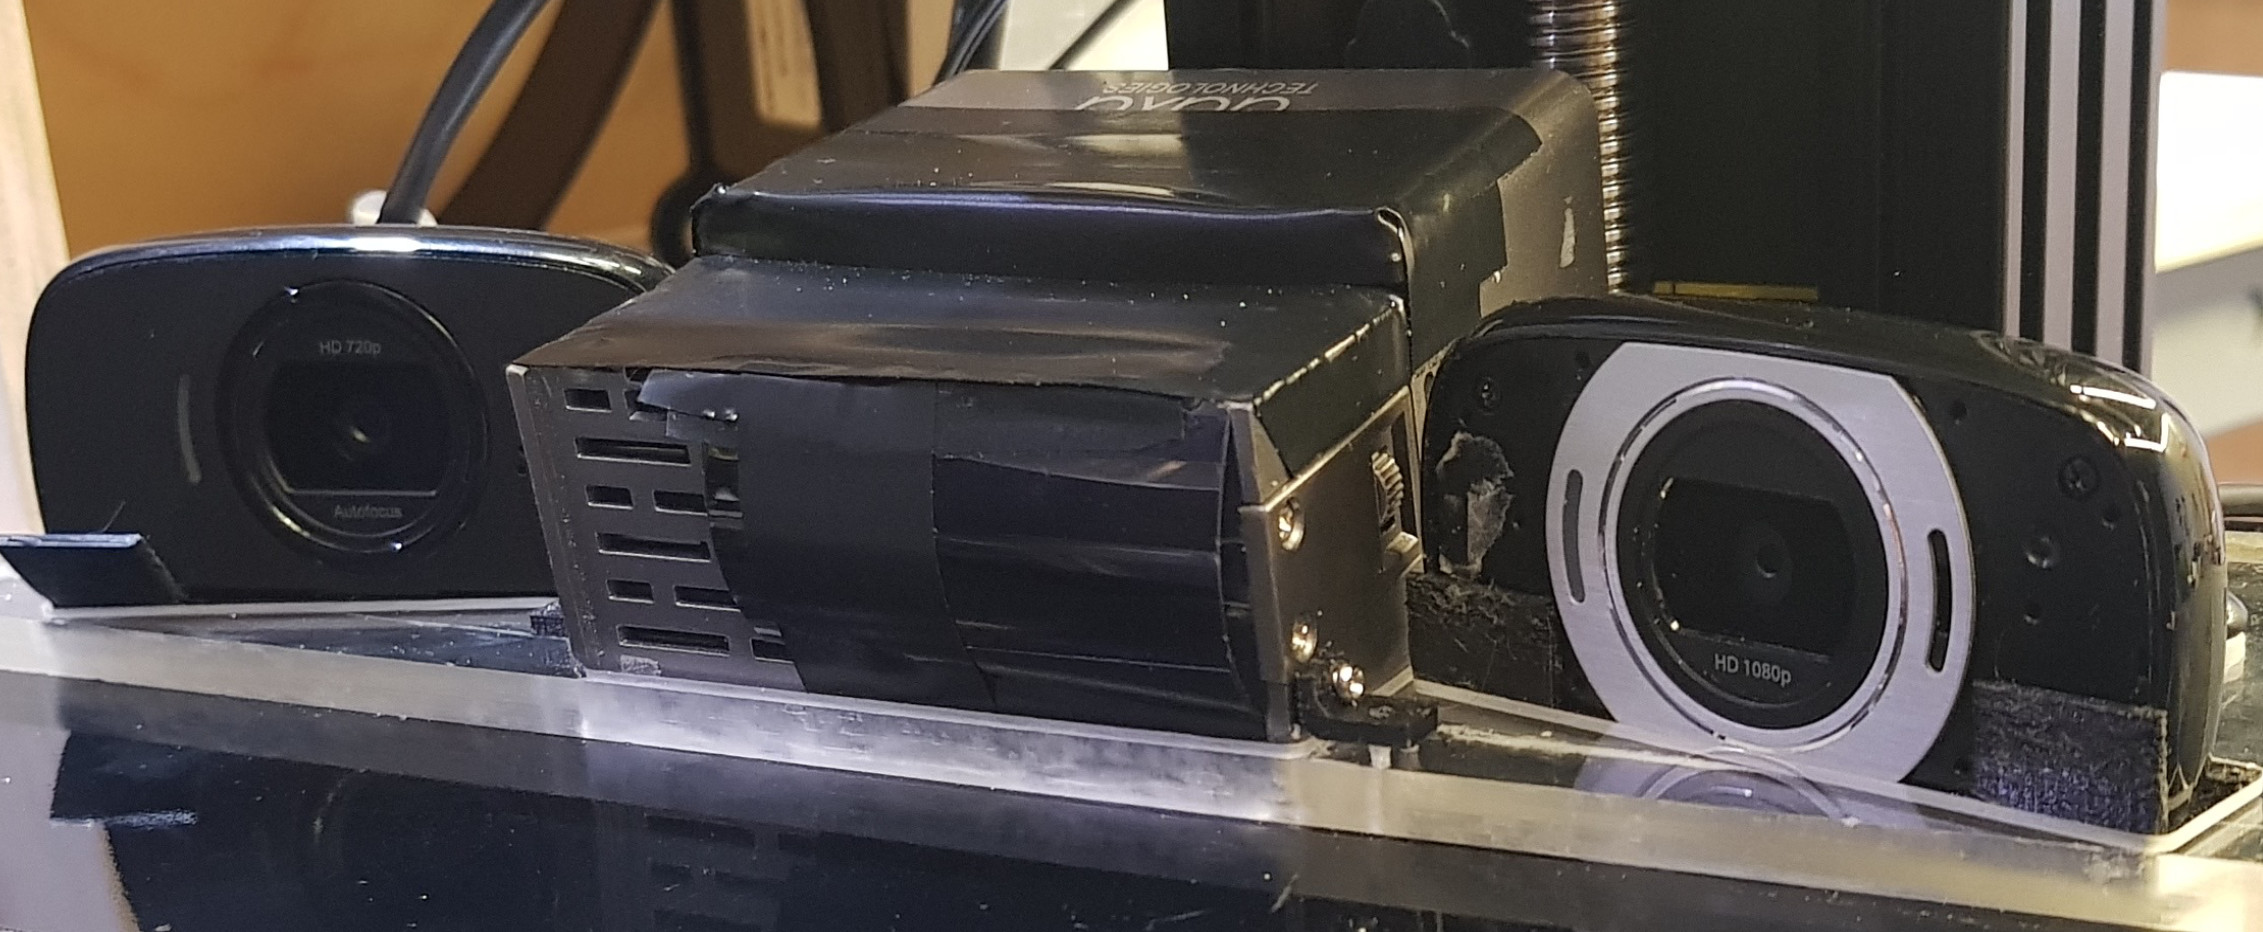
\includegraphics[height=2.4cm]{fig/omci/sli_photo.jpg}}
	\subfigure[]{\label{fig:artifact1}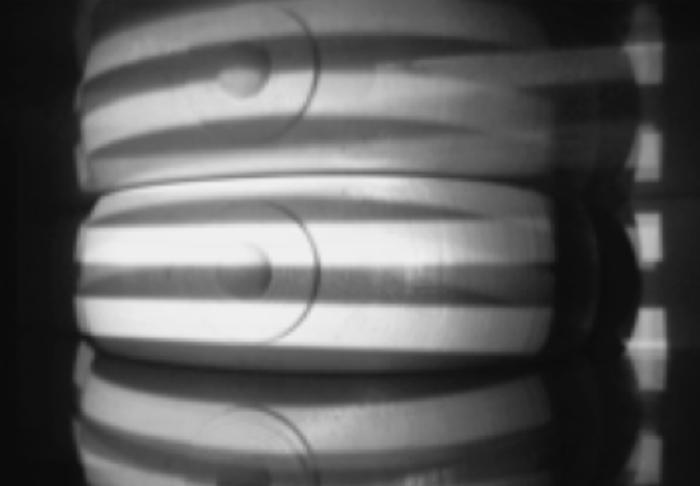
\includegraphics[height=2.4cm]{fig/omci/bars_artifact.png}}
	\subfigure[]{\label{fig:artifact2}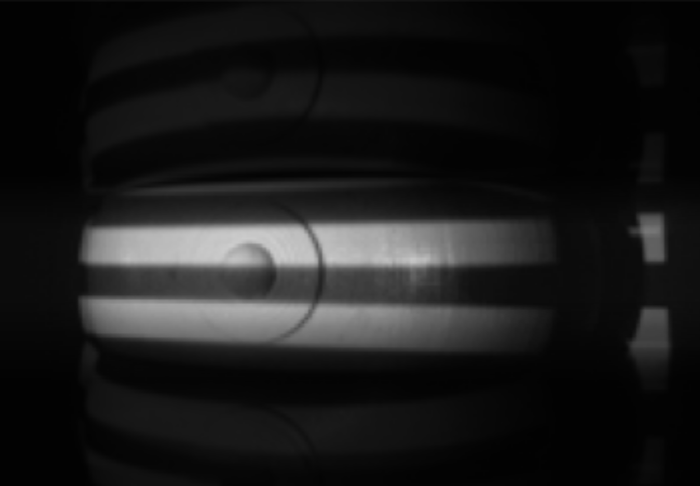
\includegraphics[height=2.4cm]{fig/omci/bars.png}}
	\end{center}
	\caption{(a) Front-view photo of the SLI system. Cameras and projectors are embedded in an acrylic mount to prevent the need for re-calibration. (b) Horizontal bar patterns reflecting off the top compression plate and onto the breast show curved illumination bar artifacts when the scaling factor $\alpha$ is set to 1. In (c), we show the same illumination pattern with thickness-informed masking eliminating the curved bar artifacts by cropping the patterns exceeding the breast surface before projection. Additionally, the scaling factor is automatically calculated to prevent camera saturation.} 
	\label{fig:barartifacts}
\end{figure} 

% encoder-informed masking
Additionally, specular reflections from the acrylic compression plates, shown in Fig.~\ref{fig:artifact1}, can produce vertically mirrored breast surfaces. To minimize such specular reflection, we use dynamic pattern masking based on real-time separation readings provided by a linear encoder. By limiting the vertical span of the illumination patterns, the patterns are projected onto the compressed breast surface without generating strong direct specular reflections from the top and bottom compression plates, as shown in Fig.~\ref{fig:artifact2}.

\subsubsection{SLI system calibration and re-projection errors}
A standard SLI camera-projector calibration is performed prior to image acquisition and is described in detail in~\cite{Moreno2012}. For each camera-projector pair, a checkerboard pattern is fully illuminated in multiple positions and the corner locations are estimated in the projector's default coordinate system using a robust pixel classification algorithm~\cite{Xu2007}. The camera and projector's intrinsic parameters (optical center and focal lengths) are estimated using a calibration method described in~\cite{Zhang2000} by fixing a world coordinate system to the calibration checkerboard plane. 

The projector's extrinsic parameters (rotation and translation from camera to projector) are calculated using a simple stereo camera calibration~\cite{Bouguet2004} that treats the projector as a secondary camera. This results in a rotation matrix and a translation vector relating the camera's coordinates to the projector's coordinates. Once the 3-D coordinates of all the corners of the checkerboard are computed using the camera's (and projector's) intrinsic and extrinsic parameters, the corners are ``reprojected'' onto all the images for which they appear. The re-projection error is defined as the average distance between the re-projected corner locations and the actual corner location. 

\subsubsection{SLI system acquisition}
The same acquisition procedures are used for both calibrating the system and acquiring breast shape measurements (Fig.~\ref{fig:sli_flowchart}). A single acquisition refers to the image capture of all illumination patterns by both cameras. Camera-projector calibration requires an acquisition at each checkerboard position. During breast measurements, the acquisition is preceded by the determination of the saturation scaling factor $\alpha$ and masking of the patterns. Patterns during calibration are not masked since the calibration is done with the system fully uncompressed. 

\begin{figure}
    \begin{center}
    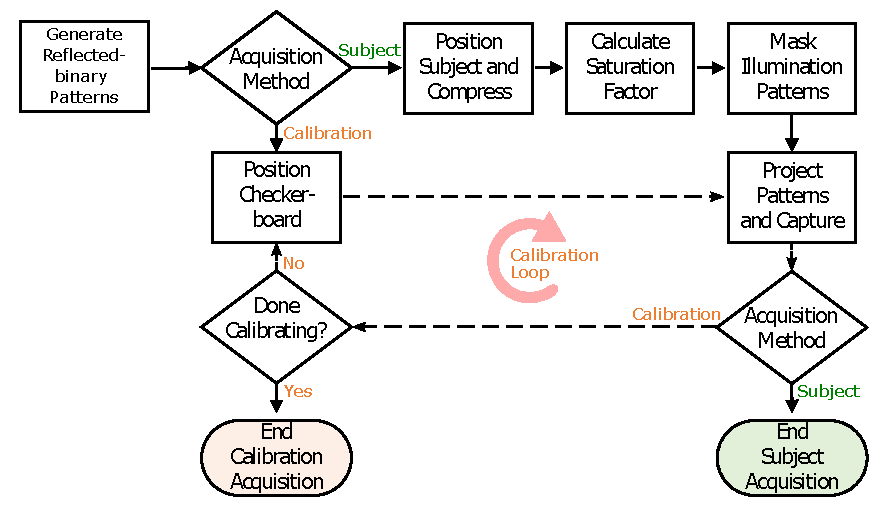
\includegraphics[width=.9\textwidth]{fig/omci/sli_flowchart.pdf}
    \end{center}
    \caption{Flow chart of image acquisition for both subject measurements and system calibration. Subject measurements calculate a saturation scaling factor and mask the illumination patterns prior to projecting patterns. System calibration measurements do not mask the illumination patterns and project at full intensity. The calibration loop (dashed lines) is repeated for each location and orientation of the calibration checkerboard.} 
    \label{fig:sli_flowchart}
\end{figure} 

%%% Subsection %%%
\subsection{Alternative breast surface reconstruction methods for assessing SLI surface accuracy}
To evaluate the accuracy of the SLI system, we compare its output against alternative surface acquisition methods. Each method estimates the surface of a 3-D breast derived from a DBT scan.

\begin{figure}
    \begin{center}
    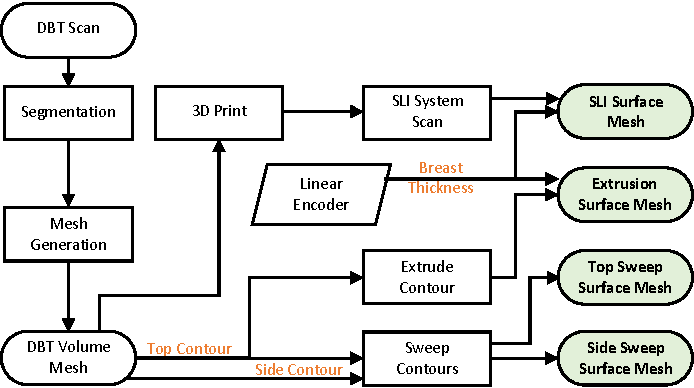
\includegraphics[width=.9\textwidth]{fig/omci/mesh_flowchart2.pdf}
    \end{center}
    \caption{Generation of breast surface meshes using multiple acquisition methods. The DBT volumetric mesh is created from segmented scans. The extrusion surface mesh is created by extruding the top contour to the breast thickness. The top and side contours of the DBT mesh are swept to create top and side surface meshes. The SLI mesh is created by scanning a 3-D printed breast phantom and trimming the resulting point-cloud using the linear encoder measurements. The surface estimation error is calculated for each of the surface meshes by comparing the surface estimations to the DBT mesh. All surface meshes are converted to volumetric meshes for validating the effect of surface estimation methods on inclusion reconstruction.}
    \label{fig:mesh_flowchart}
\end{figure} 

\subsubsection{Reference breast phantom fabrication}
Fig.~\ref{fig:mesh_flowchart} shows the process of creating surface meshes from DBT scans. Scans were obtained from radiology data from The Cancer Genome Atlas (TCGA) breast Invasive Carcinoma collection~\cite{Lingle2016}, available freely through The Cancer Imaging Archive~\cite{Clark2013}. The scan (ID: TCGA-AO-A03M) was chosen due to its large size and complex surface structure, allowing us to highlight the limitations of low field-of-view acquisition methods and as well as traditional shape estimation methods that simply sweep a single breast contour.  Digital Imaging and Communications in Medicine (DICOM) slices were segmented into breast and non-breast regions using ITK-SNAP~\cite{Yushkevich2006}. Segmented slices were converted to a volumetric image and then into a 3-D mesh using a MATLAB toolbox Iso2Mesh~\cite{Fang2009} [Fig.~\ref{fig:mesh_dbt}].

\subsubsection{Single and double contour sweep-based surfaces}
Three alternative surface estimation methods are employed in addition to the SLI surface acquisition method. These three methods use spline models of the DBT breast contours from two different planes (Fig.~\ref{fig:mammographysetup}). The extrusion method creates a surface mesh by extruding the $x/y$ breast contour in the $z$ direction to the thickness of the DBT breast measured by the linear encoder [Fig.~\ref{fig:mesh_extrude}]. The second and third methods utilize a curve-based sweep, in which a profile (shape) follows a path (contour) to create a 3-D model. In the ``top-sweep'' method, the $x/y$ breast contour profile is swept along the $y/z$ breast contour path [Fig.~\ref{fig:mesh_topsweep}]. Similarly, the ``side-sweep'' method uses the $y/z$ breast contour as the profile and the $x/y$ breast contour as the path [Fig.~\ref{fig:mesh_sidesweep}]. In both sweep methods, the profile normal is kept constant.

\begin{figure}
	\begin{center}
	\subfigure[]{\label{fig:mesh_dbt}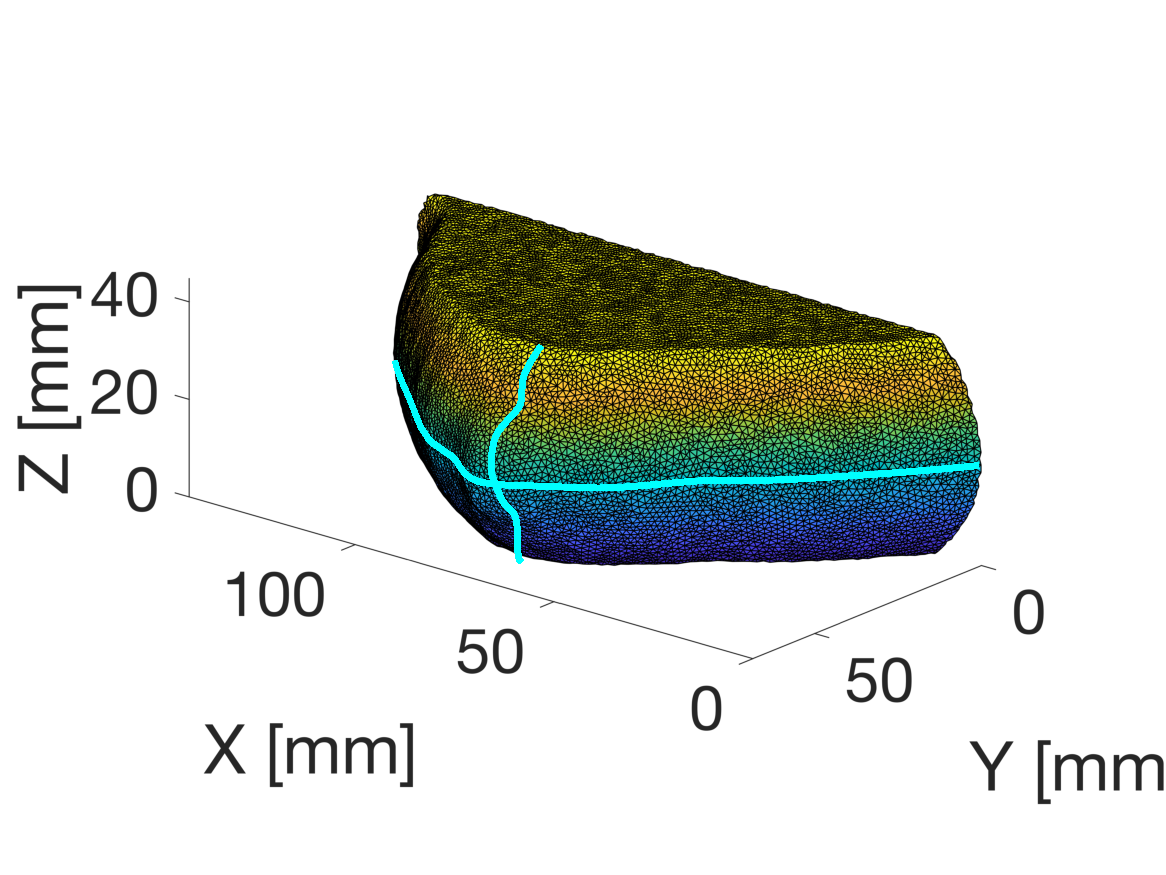
\includegraphics[width=.32\textwidth]{fig/omci/mesh_dbt.pdf}}
	\subfigure[]{\label{fig:mesh_extrude}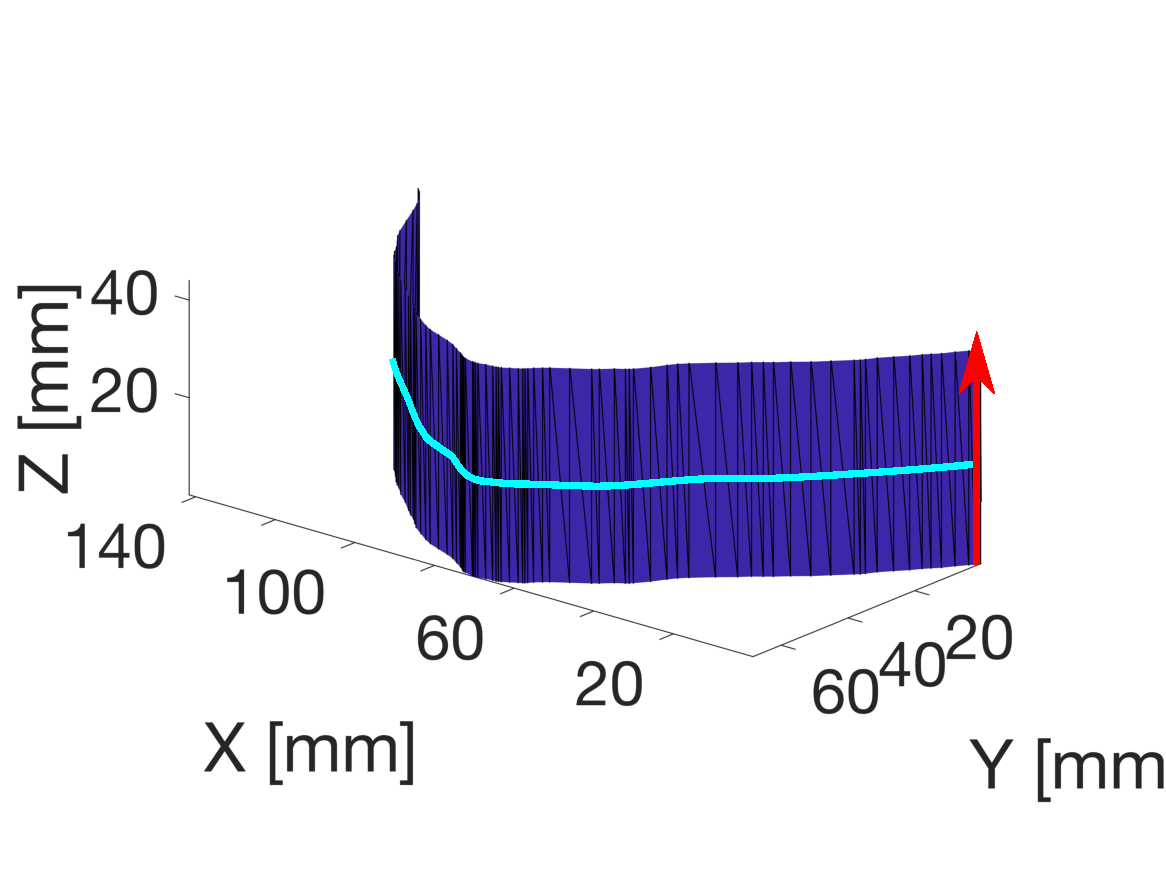
\includegraphics[width=.32\textwidth]{fig/omci/surf_ext.pdf}}
	\subfigure[]{\label{fig:mesh_topsweep}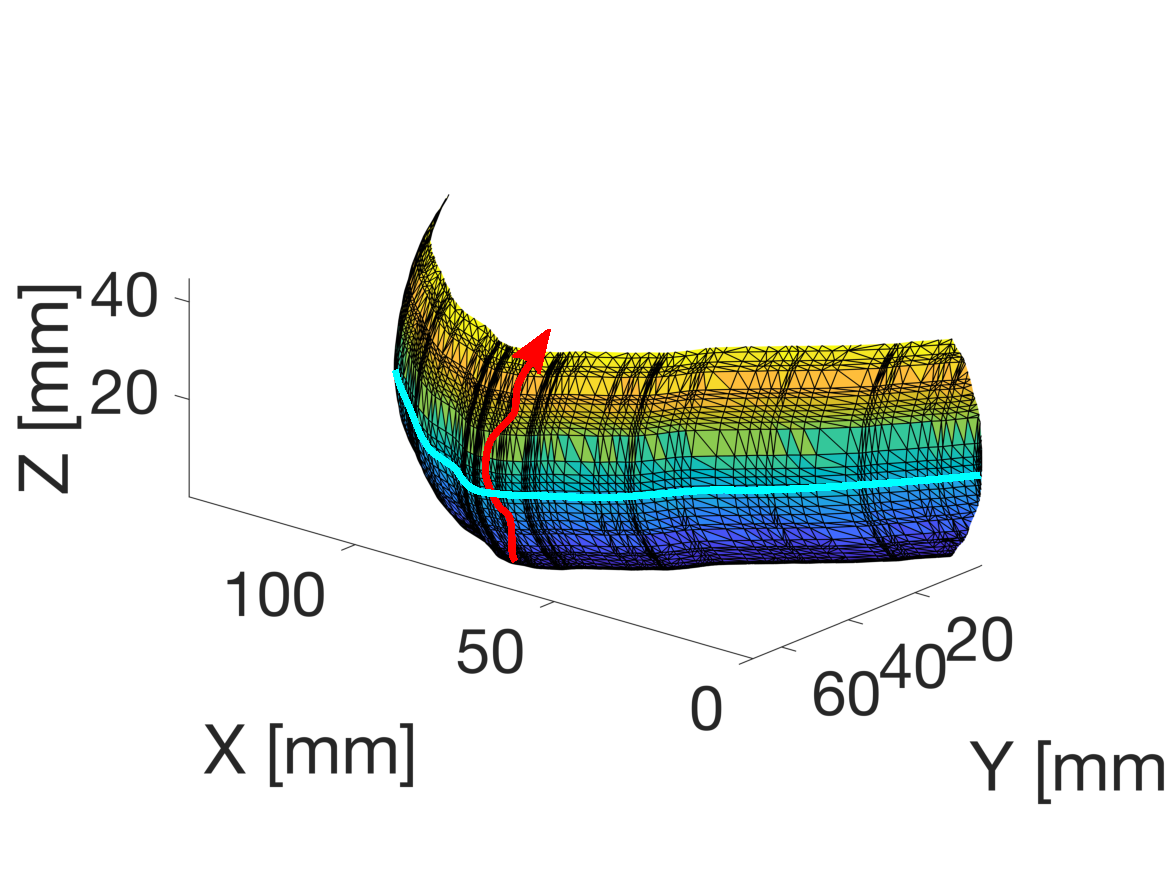
\includegraphics[width=.32\textwidth]{fig/omci/surf_top.pdf}}
	\subfigure[]{\label{fig:mesh_sidesweep}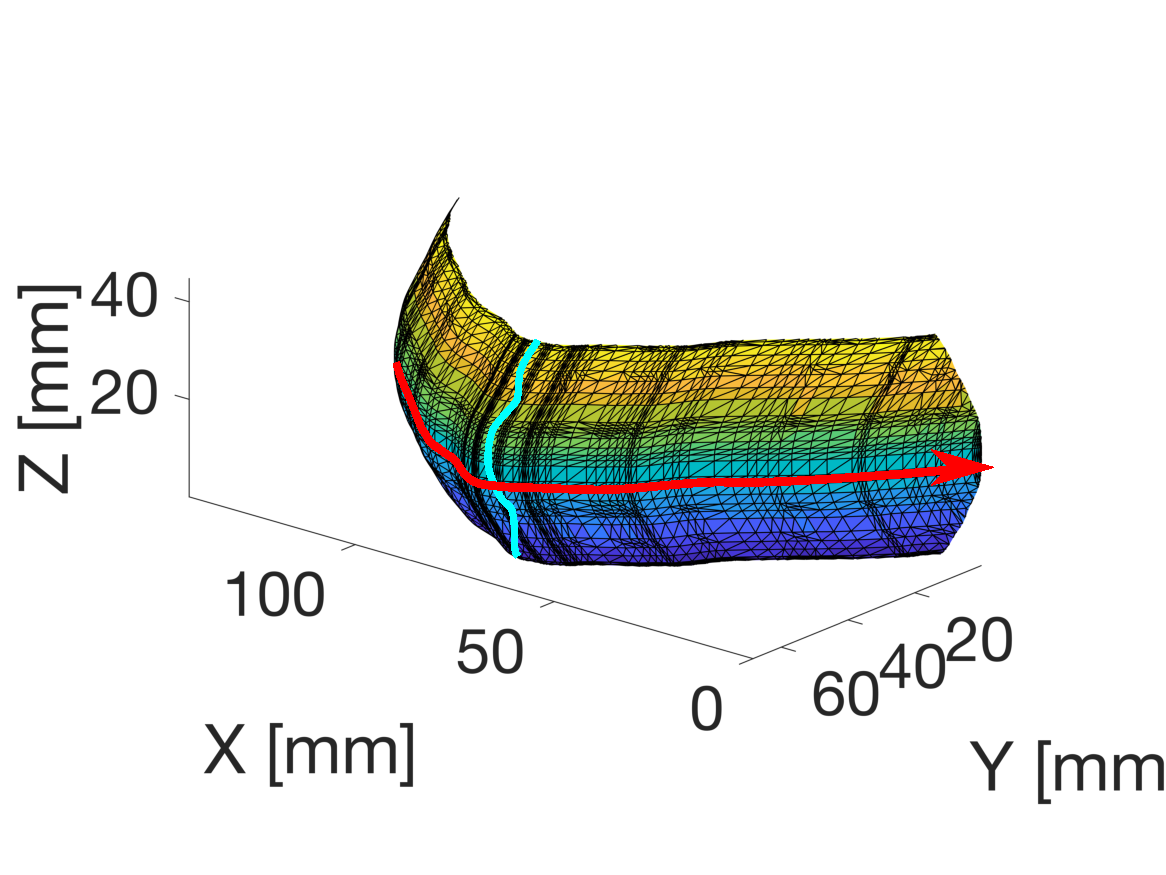
\includegraphics[width=.32\textwidth]{fig/omci/surf_side.pdf}}
	\subfigure[]{\label{fig:pcmergea}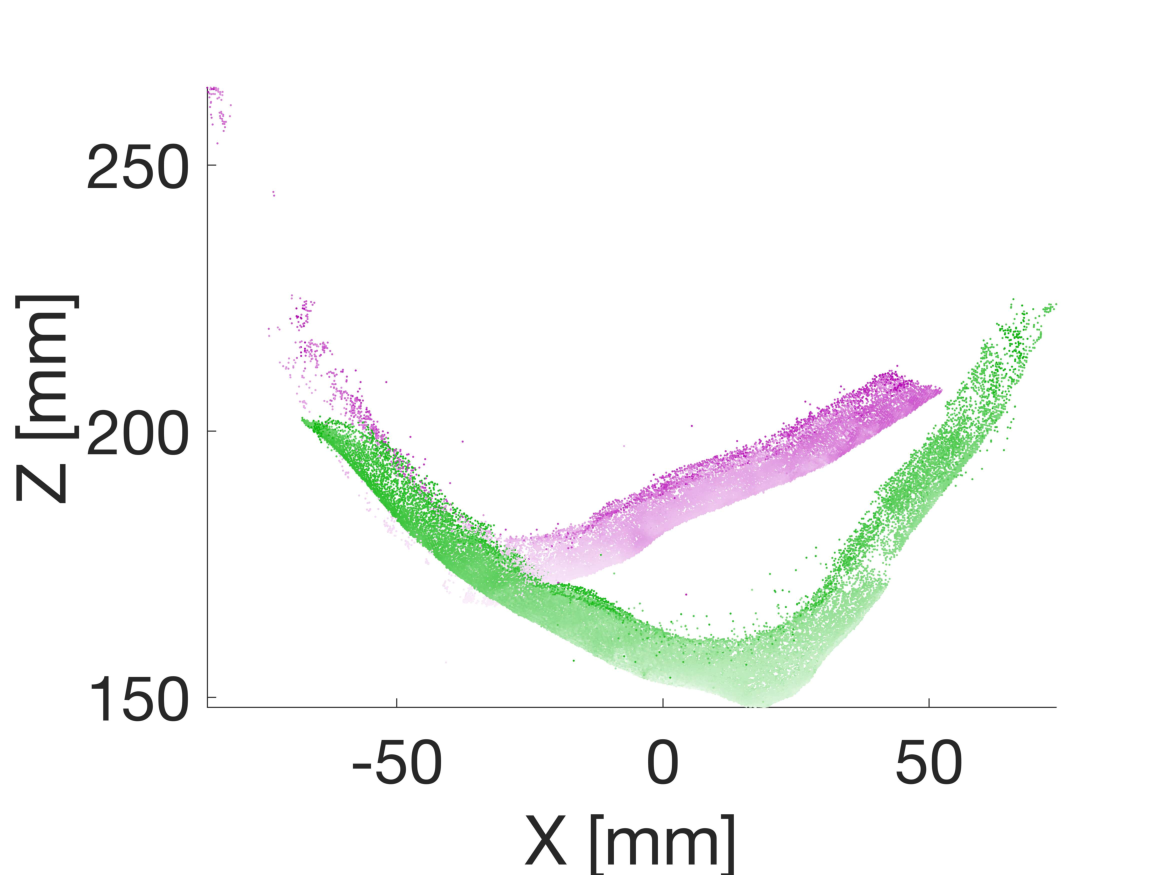
\includegraphics[width=0.32\textwidth]{fig/omci/PC_dual.pdf}}
	\subfigure[]{\label{fig:pcmergeb}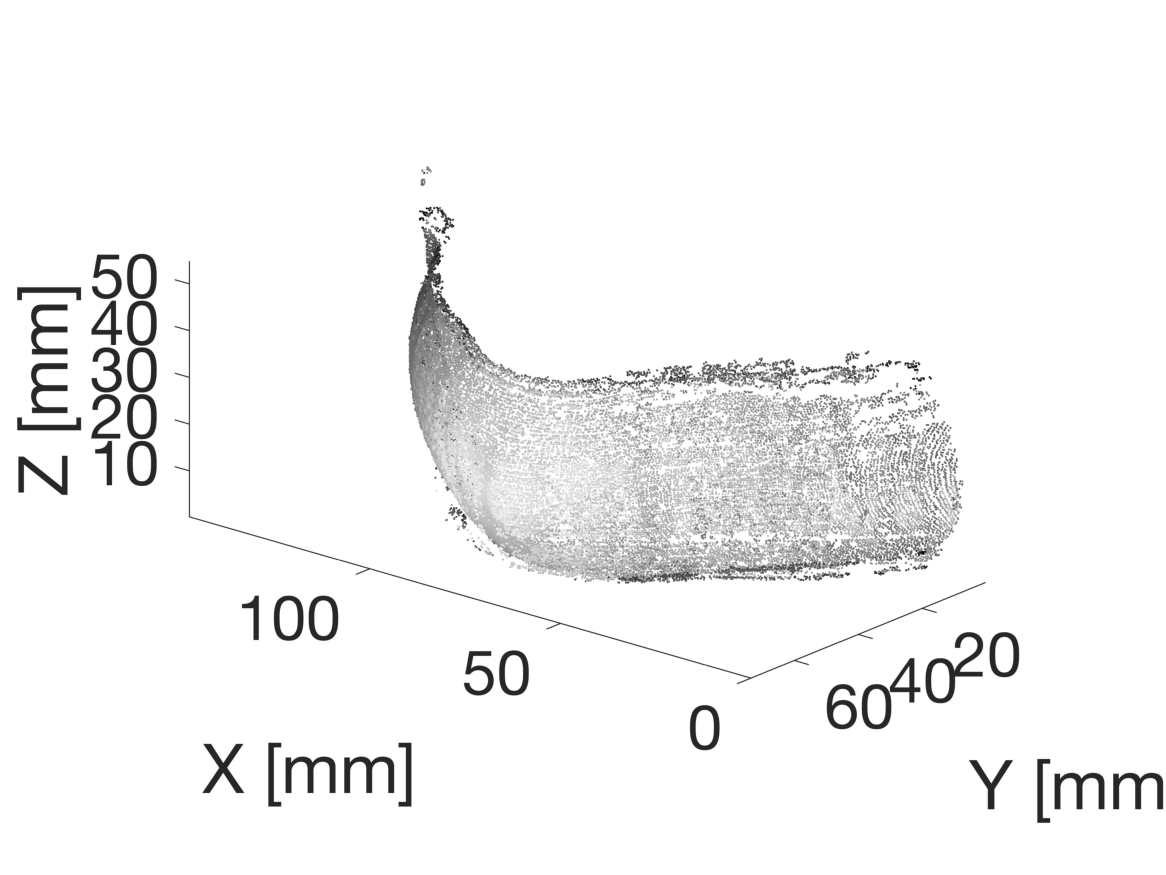
\includegraphics[width=0.32\textwidth]{fig/omci/PC_merged.pdf}}
	\end{center}
	\caption{(a) Surface mesh of a digital breast tomosynthesis model obtained from The Cancer Imaging Archive~\cite{Clark2013}. Blue cyan lines show the $x/y$ and $y/z$ breast contours from the top and side views. (b) Estimate of the DBT surface using the extrusion method in which the contour (cyan) is extruded to the thickness of the breast along the $z$ axis. (c) The top-sweep method uses the $x/y$ contour as the profile (cyan) and the $y/z$ contour as the path to sweep (red). (d) The side-sweep method uses the $y/z$ contour as the profile (cyan) and the $x/y$ contour as the path to sweep (red). (e) point-clouds from both camera-projector pairs were generated by scanning a 3-D printed model of the DBT breast using the SLI system. The green (Camera 1) and magenta (Camera 2) point-clouds are in the respective camera coordinates. (f) Merged and denoised point-cloud in the projector's coordinates.} 
	\label{fig:meshes}
\end{figure} 

\subsubsection{Structured light imaging surface mesh generation}
The SLI system estimates the surface of the compressed breast from the captured images while the breast is illuminated with Gray-code sequence patterns. Each camera-projector pair's extrinsic parameters are used to generate a point-cloud in each camera's reference frame using Scan3d-Capture~\cite{Moreno2012a} [Fig.~\ref{fig:pcmergea}]. The alignment of each camera-projector pair point-cloud is done by a rigid transformation of each point-cloud to the projector's coordinates. The point-clouds are then down-sampled using a box grid filter and merged to a single point with normal properties averaged~\cite{Pomerleau2013}. Denoising is then performed to remove outliers~\cite{Rusu2008}. The point-cloud is trimmed in the $z$ direction to the height of the DBT breast measured by the linear encoder [Fig.~\ref{fig:pcmergeb}]. The trimmed point-cloud is first converted to a mesh using a crust algorithm~\cite{Crust1999} prior to being cropped by a bounding-box mesh with height matching the breast thickness to form a closed surface mesh. 

\subsubsection{Surface estimation error}
The surface estimation error, $E_s$, of each surface estimation method is computed by comparing the nodes in each surface mesh to the nodes in the DBT mesh. The residual for each node in the surface mesh is the shortest distance from that node to the DBT mesh. The SLI output mesh is linearly translated (rotation and translation only) into the projector's frame using the projector's extrinsic parameters prior to determining residuals. $E_s$ is defined as the average residual of all nodes for a particular surface estimation method. 

%%% Subsection %%%
\subsection{Evaluation of the impact of surface errors on DOT image reconstructions}
Simulations were conducted to evaluate the impact of surface estimation accuracy on DOT reconstruction accuracy for inclusions of various depths. Breast surface meshes were converted to volumetric meshes with optical inclusions and the mean squared error of wide-field DOT reconstructions was calculated for each estimation method. 

\subsubsection{Assessment of reconstruction accuracy}
The effect of different surface estimations on lesion reconstruction was quantified using simulations of continuous wave (CW) pattern-illumination sources. A 5~mm radius spherical inclusion was added at the mid-plane of each volumetric mesh at distances of 5 to 45~mm away from the nipple. The $x$ and $z$ coordinates of the inclusion were fixed at 68 and 22~mm, respectively. The forward simulation was conducted on a ground truth volumetric mesh consisting of the DBT volumetric mesh and a spherical inclusion. The non-linear image reconstruction of tissue properties was calculated using an iterative Gauss-Newton method in which a series of corrective terms were added to an initial guess. The reconstruction resulted in distributions, $\mathrm{\mu_{a}}_{i}$, representing the resulting 3-D absorption coefficient ($\mu_a$) maps at the $i^{th}$ node for each simulated tumor location and surface model.

\subsubsection{Reconstruction error assessment}
We use mean squared error, MSE, to determine the accuracy of the image reconstruction resulting from each breast mesh. To compute the MSE, we first interpolate the reconstructed absorption map, $\mu_a$, to the DBT mesh, and then subtract the interpolated $\mu_a$ at each node $i$, with the corresponding ground truth absorption value defined on the same node, expressed as
\begin{equation}
\label{eq:mse}
\mathrm{MSE} = \frac{1}{N}\sum_{i=1}^{N}(\mathrm{\mu_{a}}_{i} - \mathrm{\mu_{a0}}_i)^{2},
\end{equation}
where $N$ is the total node number; $\mathrm{\mu_{a}}_i$ and $\mathrm{\mu_{a0}}_i$ define the recovered and ground truth $\mu_{a}$ values, respectively, at the $i^{th}$ node in the DBT mesh.


%%% Subsection %%%
\subsection{Optical phantom and patient data acquisition}
\label{Sec:DataAcquisition}
The recorded information from the three optical subsystems is supplemented by the auxiliary sensor data to obtain tomographic maps reconstructions. The data analysis pipeline that integrates all the captured information is shown in Figure~\ref{fig:DataAnalysis}. The data acquisition procedure consists of three steps. First, calibration images for each wavelength are acquired from each of the 32 sliding-bar source patterns while being projected onto a piece of paper placed over the bottom compression paddle. These images are used to locate the projection area and a realistic source pattern used during tomographic reconstruction to account for projection imperfections. Second, a reference measurement is acquired from a homogeneous optical phantom by recording images of the transmitted light when projecting each of the sliding-bar source patterns at each wavelength. Third, measurement images are acquired either from a heterogeneous phantom for system validation or from a patient breast to perform clinical measurements. A reference pattern at 660~nm is irradiated on the targeted sample to perform a iterative search of the optimum EMCCD gain value. To this end, the mean intensity over the hard-coded source pattern area in the acquired images is adjusted to be within a customized intensity-level that maximizes the signal-to-noise-ratio while avoiding saturation. This procedure is repeated for the same reference pattern irradiated at 830~nm. A solid black illumination pattern is also acquired for noise correction at the corresponding EMCCD gain value per wavelength. Next, an image of the diffuse transmitted light for each of the 32 sliding-bar projected patterns is captured using a exposure time of 200~ms. Offline post-processing of both calibration and measurement images is performed to reconstruct 3-D maps of the tissue optical properties.

\begin{figure}[]
\centering
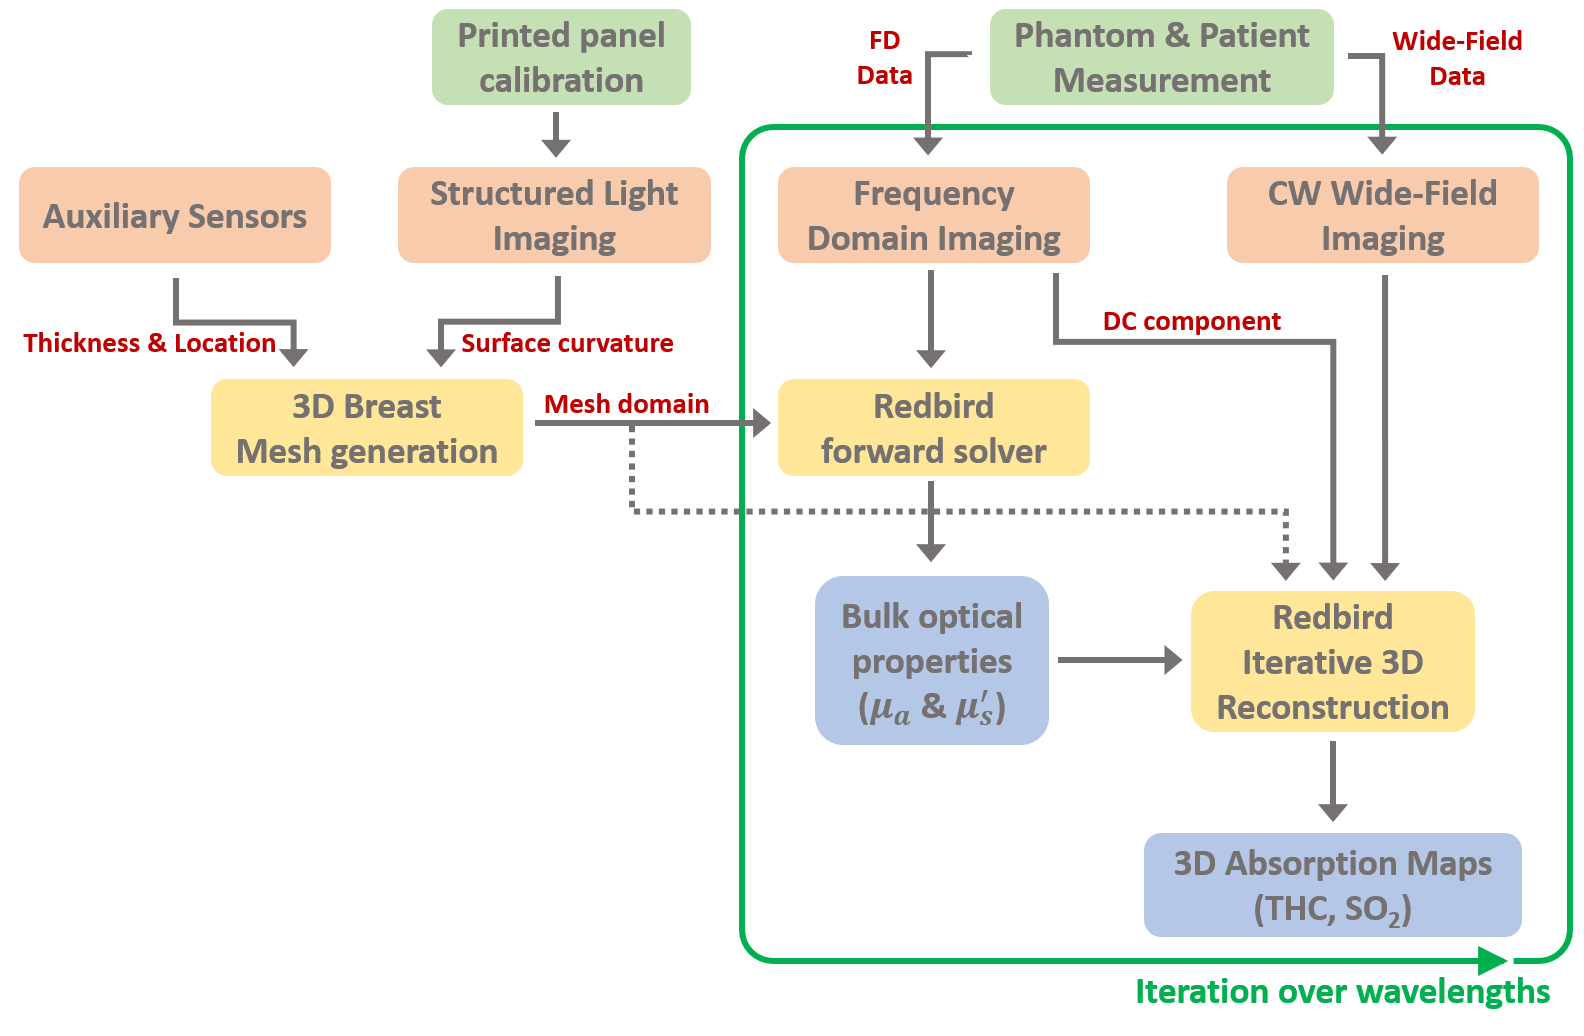
\includegraphics[width=0.90\textwidth]{fig/omci/OMCIWorkflow_280720.png}
\caption{OMCI data processing pipeline. The calibration and measurement data is fed into its corresponding processing method. The auxiliary and SLI measurements produce a 3-D breast-shaped mesh as a simulation domain. Mesh-constrained Frequency Domain (FD) analysis produces the bulk tissue optical properties of the medium. Afterwards, both the DC component of the FD data and the acquired wide-field (WF) transmission images are employed to iteratively produce tissue absorption maps. The FD and WF analysis methods are repeated over the data acquired at each measured wavelength.}
\label{fig:DataAnalysis}
\end{figure}


%%% Subsection %%%
\subsection{Three-dimensional reconstruction methods}
\label{Sec:FDanalysis}
A homogeneous phantom with known optical properties is used to calibrate the acquired optical data from the targeted samples. Two sets of tetrahedral meshes, one finer and one coarser, generated using iso2mesh toolbox~\cite{Fang2009} are used for solving the forward and inverse problems, respectively. Phantom reconstructions are based on a slab mesh whereas the clinical data uses the high-resolution breast mesh generated from the SLI system point cloud.

The calibrated frequency-domain optical measurements are used to estimate the bulk optical properties by solving the forward problem in the finer mesh using our in-house finite-element forward solver, redbird-m~\cite{Redbird2008}. This measurements serve as an initial guess in the iterative reconstruction process. Single pixel values~\cite{Yao2015} are computed as the dot product of the the captured wide-field transmission images and a 32$\times$ sliding-bar pattern (same as the source). Inverse problem of the diffusion approximation in the coarse mesh is solved by using an iterative Tikhonov-regularized Gauss-Newton method over 15 iterations. A finer representation of the reconstructed three-dimensional distribution of tissue physiology are obtained by mapping the coarser and finer meshes.



\section{Results}
\label{chap:omci:results}
Here, we will report the results from the frequency domain and wide-field subsystems first. The SLI results section will be broken down into three parts. We will first report the projector and camera re-projection errors of our SLI calibration using the calibration checkerboard. We then quantify the error of surface estimation methods in estimating the surface shape of the DBT breast. Finally, we show the effect of different surface estimation methods on optical property reconstruction using simulations of continuous wave pattern-illumination sources. Once all subsystems are characterized individually, we will show patient results from a full system measurement.


%%% Subsection %%%
\subsection{Frequency-domain subsystem characterization}
\begin{figure}[]
    \begin{center}
    \subfigure[]{\label{fig:RFSystemA}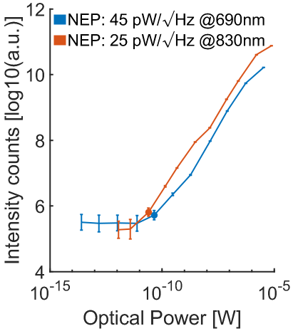
\includegraphics[width=.35\textwidth]{fig/omci/RFCharacterizationA.png}}
    \subfigure[]{\label{fig:RFSystemB}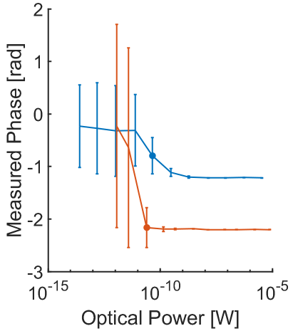
\includegraphics[width=.35\textwidth]{fig/omci/RFCharacterizationB.png}}
    \end{center}
    \caption{Frequency domain subsystem characterization.} 
    \label{fig:RFSystem}
\end{figure} 

A motorized multi-level attenuation filter wheel was used to characterize the dynamic range of the designed galvo-based frequency-domain subsystem. A noise equivalent power (NEP), the signal power that gives a signal-to-noise ratio of one in a one hertz output bandwidth, lower than 45~pW$/\sqrt{Hz}$ and 25~pW$/\sqrt{Hz}$ were obtained for 690~nm and 830~nm source wavelengths, respectively. A dynamic range greater than 100~dB (20log10) for both wavelengths was characterized when reaching the saturation level of the detection sensor at 1.5~mW (Figure.~\ref{fig:RFSystemA}). The phase noise was quantified to be less than 10~mrad in each wavelength at optical powers higher than the NEP (Figure.~\ref{fig:RFSystemB}). Finally, the system stability was assessed over a time period of 4 hours when irradiating light sources of 1~mW at each wavelength. No inter-wavelength or amplitude-to-phase crosstalk was observed during data acquisition.


%%% Subsection %%%
\subsection{Continuous wave wide-field subsystem characterization}
A homogeneous silicon phantom slab was used to characterize the continuous wave wide-field system. A set of 32 sliding-bar patterns were projected onto the bottom surface of the phantom whereas the same pattern set was employed as digital detectors to mask the collected diffuse transmittance images (10 images per pattern, 320 images in total) as in single-pixel detection method~\cite{Pian2015}. The SNR was computed for the coupling of each source-detector pair and observed to range from 55 to 87~dB at 660~nm and from 56 to 74~dB at 830~nm. Wide-field system stability was assessed over a period of 4 hours per wavelength by projecting a fully illuminated pattern over the homogeneous phantom bottom surface. Images of the transmitted light were acquired at a 5 frames-per-minute pace (a total of 1200 images) to evaluate the intensity fluctuations due to ambient temperature and light source current control variability. Intensity variations $<$5\% in both wavelengths were observed during the evaluated time period.

A heterogenous phantom was use...
Optical contrast of inclusion (2 and 4x contrast), size of phantom (8x15x4.5cm), spherical inclusion size (1.5 and 2.5~cm diameters).
Number of patterns illuminated (32 patterns). 
Number of iterations (15).
FWHM shown. at y=4cm.


1.5 and 2.5~cm diameters

\begin{figure}[]
    \begin{center}
    \subfigure[]{\label{fig:PhantomResultsA}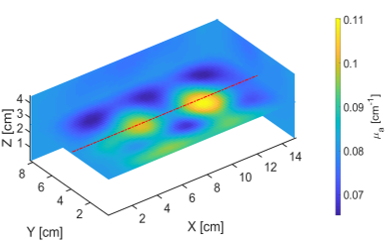
\includegraphics[width=.4\textwidth]{fig/omci/PhantomResultsA.png}}
    \subfigure[]{\label{fig:PhantomResultsB}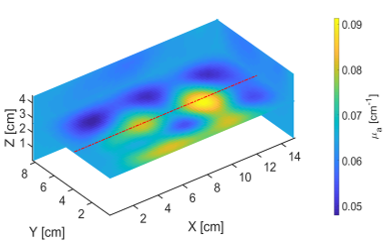
\includegraphics[width=.4\textwidth]{fig/omci/PhantomResultsB.png}}
    \subfigure[]{\label{fig:PhantomResultsC}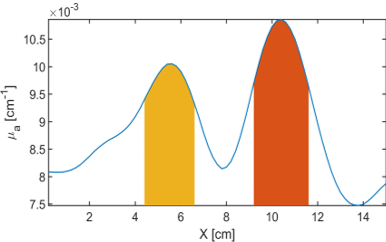
\includegraphics[width=.4\textwidth]{fig/omci/PhantomResultsC.png}}
    \subfigure[]{\label{fig:PhantomResultsD}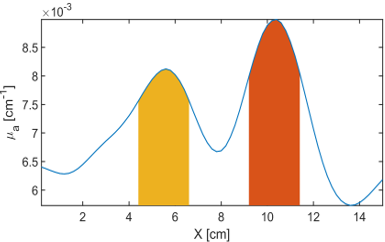
\includegraphics[width=.4\textwidth]{fig/omci/PhantomResultsD.png}}
    \end{center}
    \caption{OMCI \textit{in-vitro} validation at two wavelengths (columns). Localization of two absorption contrast (2x and 4x) inclusions. The recovered inclusion sizes of 2.1 cm and 3 cm (shaded area) denote an over estimation of about 0.5 cm with respect to the real inclusion size.} 
    \label{fig:PhantomResults}
\end{figure} 



%%% Subsection %%%
\subsection{SLI subsystem characterization}


\subsubsection{Camera-projector calibration and surface acquisition}
\label{ssec:calibrationresults}
Our dual-camera SLI system was calibrated in a dark room using a checkerboard with 5$\times$7 internal corners with 1$\times$1~cm$^2$ black and white squares. The calibration checkerboard was printed and adhered to a black Delrin surface to ensure it remained planar. To account for varying breast shapes and curvatures, the checkerboard was placed at 7 locations. At each location, camera images were captured for 5 board orientations: 1) normal to the $y$-axis [see Fig.~\ref{fig:mammography_top}], 2) rotated left and 3) rotated right by 30 degrees relative to the $x$-axis, and 4) tilted forward and 5) tilted backward by 30 degrees in the $y/z$ plane [Fig.~\ref{fig:mammography_side}]. This results in a total of $7\times5=35$ checkerboard positions within the camera and projector field-of-views (Fig.~\ref{fig:mammographysetup}). Each rotation and tilt was measured manually using a printed protractor. The projector's resolution is 1280$\times$720 pixels and the resolution of the cameras is 1600$\times$896 pixels. Using a Gray-code of bit-length $P=9$, we acquire $P\times 4 + 2 = 38$ images (see Section~\ref{sec:sli}) at each board orientation/position placement. An exposure time of 0.25 seconds per image per camera results in a total one-time calibration time of $38 \times 7 \times 5 \times 2 \times 0.25 = 665$ seconds. The first camera-projector pair (Camera 1 with projector) resulted in a camera and projector re-projection error of 0.4089 and 0.2282 pixels, respectively. The second camera-projector pair resulted in a camera re-projection error of 0.4368 pixels and a projector re-projection error of 0.2889 pixels.

A re-calibration is only necessary when the relative position of the cameras and projector is changed. Once calibrated, the SLI system can acquire a surface scan in about 35 seconds, including 16 seconds for adaptively adjusting the intensity scaling factor $\alpha$ for both cameras (see Section~\ref{sec:special} for details) and 19 seconds for image acquisition ($38 \times 2\times 0.25 = 19$ s).

%%% Subsection %%%
\subsubsection{Surface estimation errors}
\begin{table}
    \centering
    \caption{Mean and standard deviation of the residuals of each point in a surface estimation mesh compared to the original DBT breast mesh.}
    %\resizebox{\textwidth}{!}{%
        \begin{tabular}{lcccc}
        \toprule
         & Extrusion & Top-Sweep & Side-Sweep & SLI \\ \midrule
        Surface estimation error, $E_s$ [mm] & 6.8353 & 0.3772 & 0.4726 & \multicolumn{1}{l}{0.2543} \\
        Standard deviation [mm] & 2.8671 & 0.3029 & 0.3370 & 0.2723 \\ \bottomrule
        \end{tabular}%
    %}
    \label{tab:residuals}
\end{table}

The DBT breast model was 3-D printed (Ender 5, Creality, China) with a 0.1~mm layer height using white polylactic acid (PLA) filament. The 3-D printed DBT breast was placed in between the compression plates, compressed to the thickness of the printed DBT phantom, and scanned using the dual-camera SLI system. The saturation scaling factors $\alpha$ were automatically determined using twenty iterations, resulting in a $\alpha=0.8$ for both cameras. The two point-clouds from each camera-projector pair were transformed to the projector's coordinates, down-sampled, and merged prior to being denoised with the number of nearest neighbor points set to four and the outlier threshold set to one standard deviation from the mean of the average distance to those four neighboring points. The resulting point-cloud from the SLI system scan has 35,256 points.

Table~\ref{tab:residuals} shows the mean and standard deviation of the residual of all the nodes in the estimated breast surface mesh. The $z$-extrusion method (EXT) results in the largest error ($E_s$) of all compared methods. While the top-sweep, side-sweep, and SLI methods all had similar standard deviations, the SLI method resulted in the smallest $E_s$.

%%% Subsection %%%
\subsubsection{Mean square error of optical property reconstruction}
\begin{figure}
	\begin{center}
	    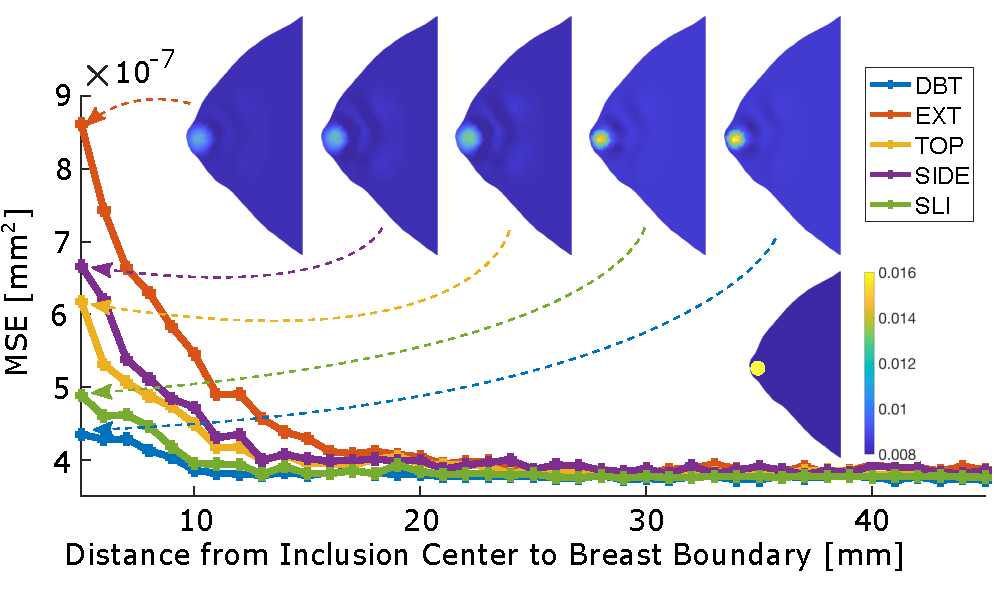
\includegraphics[width=.9\textwidth]{fig/omci/mse.pdf}
	\end{center}
	\caption{A comparison between the mean squared error (MSE) of the reconstructed absorption map using 4 estimated surfaces (EXT - $z$-axis extrusion, TOP - sweeping $x/y$ contour along $y/z$ contour, SIDE -- sweeping $y/z$ contour along $x/y$ contour, and SLI -- surface acquired from our SLI system) as well as the ground truth surface (DBT). A 1~cm diameter spherical inclusion is moved away from the breast surface at various depths between 5 and 45~mm in 1 mm increments. Image slices (in $x/y$ plane) of the reconstructed absorption coefficient ($\mu_a$ in mm$^{-1}$) (top-row) and the ground truth $\mu_a$ (bottom-right) are shown as insets.}
	\label{fig:mse}
\end{figure} 

DOT reconstructions were performed using our in-house data analysis toolbox, Redbird-m~\cite{Redbird2008}. An $L$-curve analysis is used to determine the regularization parameter as $3.16\times 10^{-10}$, which is fixed over 10 Gauss-Newton iterations. The absorption coefficient of the spherical inclusion was set to be twice ($\mu_a=0.016$/mm) that of the background tissue ($\mu_a=0.008$/mm). The reduced scattering coefficient $\mu_s'$ was set to $1$~mm$^{-1}$ for both breast and inclusion tissues. A set of 32 (16 vertical, 16 horizontal) moving-bar source patterns~\cite{Yao2015} covering an area of 40$\times$40~mm$^2$ was centered at the spherical inclusion. Iso2Mesh was used to interpolate nodal values from the reconstructed mesh to the ground truth mesh based on linear interpolation in order for all reconstructed meshes to have the same number of nodes.

The MSE errors from these reconstructed images are summarized in Fig.~\ref{fig:mse}, showing the effect of different surface estimation methods on the accuracy of optical property recovery. Overall, surface mesh accuracy appears to have a notable impact on relatively shallow tumors, with a depth of less than 25~mm. MSE values obtained using the SLI method closely follow those using the ground truth DBT mesh for most inclusion depths. The top- and side-sweep-based meshes followed similar trends, however, reporting higher errors compared to SLI especially when the tumor is relatively shallow. The maximum MSE value for the SLI mesh at a distance of 5~mm from the surface ($4.89\times 10^{-7}$~mm$^2$) was 23\% higher than the maximum MSE value for the DBT mesh ($4.35\times 10^{-7}$~mm$^2$). In contrast, the single-axis-extrusion method (EXT) MSE was nearly twice higher ($8.62\times 10^{-7}$ mm$^2$) than that from the DBT mesh. Although the DBT and SLI mesh MSEs plateau to their minimum around 15~mm from the surface, top-, side-, and extrusion-based mesh MSEs continue to decrease until a depth of 25~mm. Beyond the depth of 25 mm, the errors between different methods become minimal.

\subsection{full system in-vivo patient results}
\begin{figure}[]
    \begin{center}
    \subfigure[]{\label{fig:PatientResultsA}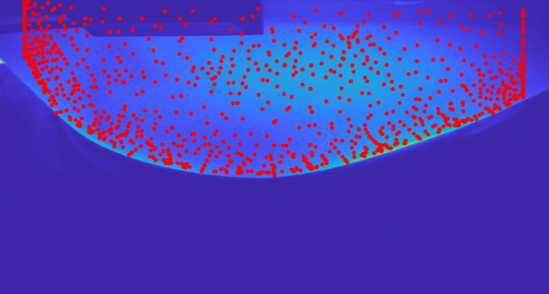
\includegraphics[width=.4\textwidth]{fig/omci/SLIMeshC.png}}
    \subfigure[]{\label{fig:PatientResultsB}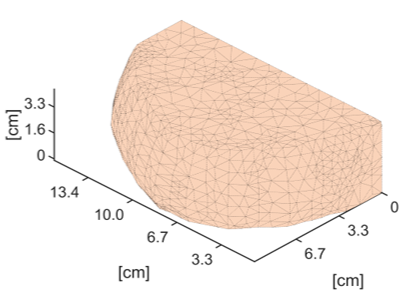
\includegraphics[width=.4\textwidth]{fig/omci/SLIMeshD.png}}
    \subfigure[]{\label{fig:PatientResultsC}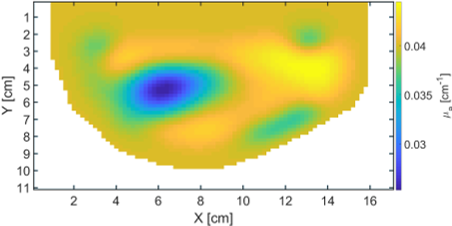
\includegraphics[width=.4\textwidth]{fig/omci/PatientResultsA.png}}
    \subfigure[]{\label{fig:PatientResultsD}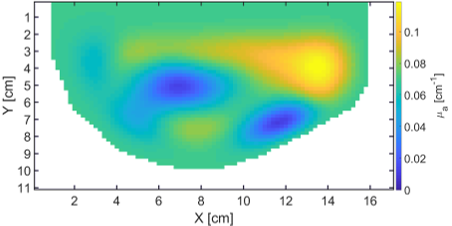
\includegraphics[width=.4\textwidth]{fig/omci/PatientResultsB.png}}
    \end{center}
    \caption{(a) The recovered point cloud from a patient measurement conforming to the breast curvature. (c) The generated 3D breast-shaped mesh from a SLI measurement on a healthy patient. (c-d) OMCI \textit{in-vivo} validation at two wavelengths. Recovered breast structures from a healthy patient corresponding to the axilla muscle, adipose tissue and fibroglandular structures.} 
    \label{fig:PatientResults}
\end{figure} 

%Danvers, IRB approved, healthy subject, prior x-ray within X months.
%Acquisition time, time in compression for each breast. 
%Make sure patient we choose has a nipple (so we can see the SLI recovery). 
%Find a patient with registered data. 



\section{Discussion}
\label{chap:omci:discussion}

% FD results
Our multi-distance and multi-wavelength frequency domain spectroscopy subsystem provides an accurate decoupling of the bulk tissue optical properties. By using a multi-distance and dual-wavelength approach, our FD subsystem provides accurate optical properties, even in the presence of tissue heterogeneities. Encoder-informed compression allows the FD subsystem to automatically derive source-detector distances and adjust for varying compression thicknesses. The use of galvo-based positioning allows our FD system to easily adapt to breasts of varying sizes or localized heterogeneities through either higher resolution positioning within a single axis or through the use of multiple axes for calculating bulk optical properties from larger areas. Although currently limited to a single degree of freedom, the characterization of the FD subsystem resulted long-term stable NEP and dynamic range comparable to existing DOT systems (Figure~\ref{fig:RFSystem}).  

% WF results
Our high-density wide-field light source combined with a camera-based detection of the diffuse transmitted light through the compressed breast allows us to obtain high-density spatial sampling and accelerated data acquisition all while bypassing traditional optical coupling coefficients artifacts. The \textit{in-vitro} validation in Figure~\ref{fig:PhantomResults} demonstrate this subsystem's ability to reconstruct the size and optical properties of spherical inclusions from a heterogeneous phantom. The phantom had a set of two- and four-fold absorption contrast inclusions (1.5 and 2.5~cm diameters) embedded inside a homogeneous media. The reconstructed inclusions were observed to be under estimated by a two-fold difference optical contrast while the inclusion sizes were over estimated by 20\%. Additionally, the recovered bulk optical properties of the homogeneous media using the FD subsystem matched the ground truth values.  

% SLI results - reprojection errors
The camera and projector re-projection errors in Section~\ref{ssec:calibrationresults} represent an average error of less than 0.5 pixels in estimating the corner locations of a calibration checkerboard placed between 50 and 250~mm away [Fig.~\ref{fig:mammography_side}] from the projector for all 35 checkerboard positions. Although the same illumination patterns and calibration checkerboard positions were used to calibrate each camera-projector pair, we find a slightly better calibration accuracy when the projector is paired with Camera 1 since Camera 1 is closer to the projector's lens (Fig.~\ref{fig:mammographysetup}). The discrepancy in the re-projection errors of the two pairs is due in part to the asymmetry of the dual-camera setup. The asymmetry arises from the projector offset relative to its housing, making one camera closer to the projector than the other [Fig.~\ref{fig:mammography_top}]. 

% SLI results - surface errors
From Table~\ref{tab:residuals}, the single-axis extrusion method resulted in the highest surface error because it does not account for the curvature of the breast in the $y/z$ plane [Fig.~\ref{fig:mesh_extrude}]. Table~\ref{tab:residuals} indicates that, on average, points in the extrusion-method-derived surface estimation mesh are approximately 6.84~mm away from the DBT mesh. The top- and side-sweep methods decrease the surface estimation error by incorporating a second breast contour from the $y/z$ plane [Figs.~\ref{fig:mesh_topsweep} and \ref{fig:mesh_sidesweep}]. Both methods improve the accuracy of surface estimations by approximating the 3-D curvature of the breast. We want to point out that both top-sweep and side-sweep methods require an additional camera to obtain two orthogonal views of the breast~\cite{Pinto2020}, which does not necessarily lead to simplified hardware compared to the SLI setup considering the mounting space constraints and lighting conditions~\cite{Rodriguez2017}. While also requiring two cameras, our mammography-tailored SLI system can produce sub-millimeter resolution of the surface compared to the reference DBT breast model based on Table~\ref{tab:residuals}.

% SLI results - MSE
Our results also demonstrated that the improvement in surface estimation accuracy can lead to improved DOT reconstruction accuracy. Fig.~\ref{fig:mse} shows using breast surfaces derived from SLI can accurately recover the absorption profile compared to those recovered using the ground-truth (DBT) mesh at most tested tumor depths. For superficial/shallow ($<$ 10~mm) tumors, the top- and side-sweep surface estimation methods followed similar trends to each other, reporting MSEs about 50\% higher compared to those from using ground-truth (DBT) surface models, and about 30\% higher than those from using SLI surfaces. As expected, the effect of the surface accuracy decreases as the inclusion is moving further away ($>$ 25~mm) from the skin.

% Patient results
In addition to the characterization of subsystems above, the complete OMCI system has also been successfully validated \textit{in-vivo}. In patient measurements, the SLI subsystem successfully adjusted its projector intensity to prevent webcam saturation. The recovered bulk breast tissue optical properties from the FD subsystem followed the reported values from our group~\cite{Fang2009} and others~\cite{Durduran2002}. Moreover, the 3-D reconstruction of the tissue physiology parameters resembles the internal breast tissue structures (i.e. adipose, muscle and fibroglandular tissue) described previously~\cite{Fang2009}, denoting the capability of our system to resolve breast compounds.

%limitations
Focusing on the SLI subsystem, despite the ability to produce sub-millimeter resolution of breast surfaces in poorly lit and confined mammography-like settings, both our SLI system and our analysis have limitations. Firstly, the span of the output point-cloud from our SLI system is limited to the area of the breast that is well-illuminated by the projector. As a result, tissue boundaries near the chest wall or those in direct contact with the compression plate may not be well covered due to the limited angles of the projector/camera line-of-sight. Still, for DOT of a compressed breast, capturing a significant portion of the front-facing breast tissue as our system does, provides quantitative differences in reconstructions, as shown above. Future improvement of this system should consider using more compact, wide-angle projectors, higher resolution cameras, and patterns with higher order binary codes to both expand the field-of-view and increase the point-cloud resolution. Secondly, a 3-D printed breast model was used to experimentally compare different shape acquisition methods. Different choices of extruder sizes, filament colors, and printing techniques could impact the surface texture of the printed phantom and slightly alter the surface estimation errors. Finally, the quantification of reconstruction errors was based on simulations using a single set of pre-determined breast models, tumor size and shape, tumor contrast, and wide-field pattern size. An experimental validation using heterogeneous phantoms may produce more realistic comparisons.

In general, even though our current setup consists of a dual-wavelength approach for tomographic reconstruction of HbT and HbO$_2$ tissue parameters, further integration of other wavelength is readily accessible, which may lead to improved physiological characterization. Moreover, frequency multiplexing of multiple illumination wavelengths can be exploited in order to accelerate optical data acquisition as recently reported by Applegate et.al~\cite{Applegate2017}. In this regard, although our current OMCI data acquisition frame rate of 2~Hz is two times faster than our previous system~\cite{Zimmermann2017}, we anticipate that future implementations of multiplexed illumination will further accelerate our framework. In addition, the implementation of a low-latency projector could also enhance the performance of our system. 

Besides these technical improvements, we foresee the capability of simultaneously retrieving the bulk tissue optical properties from the collected optical data through the implementation of a compact scientific camera in the imaging compartment below the bottom compression paddle. Furthermore, this reflectance-based approach can also be extrapolated to the structured light imaging (SLI) subsystem, by which, the collected diffuse reflected light can also be utilized for estimating the breast tissue optical properties. In addition, recording and further integration of the laterally diffused transmitted light can potentially be embedded into the reconstruction algorithm to better constrain the inverse problem in the Z-axis, thereby improving the spatial registration of the detected breast lesions. Finally, a digital single-pixel data processing approach~\cite{Belanger2010,Pian2015} may provide us the flexibility to explore several other mechanisms for subtracting quantitative information. In this work we explored the usage of low-frequency source and detection patterns for illumination and detection, respectively. Our selection was based on the fact that it has been shown that tissue acts as a low-pass filter~\cite{OSullivan2012}, hence high frequency patterns might potentially lead to a loss of information. In this regard, a future exploration on this topic has to be performed in order to obtain insights about the optimum source-detection patterns.


% CONCLUSION GOES INTO THE CONLUSION OF THE ENTIRE THESIS

% --- EOF ---